\subsubsubsubsection{Moveable agent}
\begin{figure}[h]
\centering
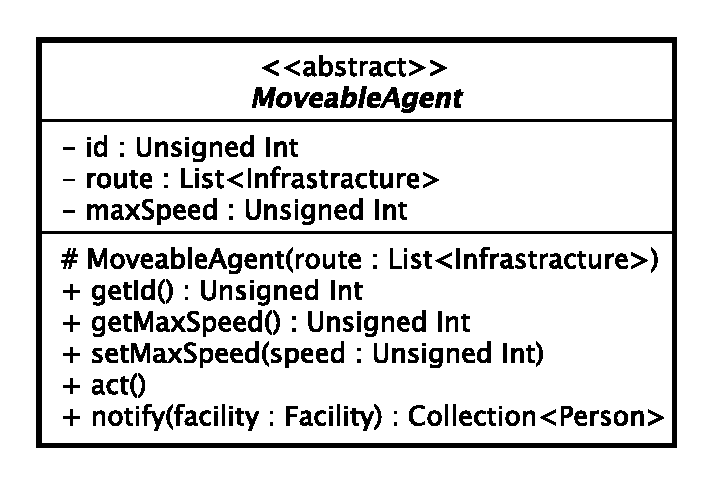
\includegraphics[scale=0.6,keepaspectratio]{images/solution/app/backend/moveable_agent.eps}
\caption{\pActive::MoveableAgent}
\label{fig:sd-app-moveable-agent}
\end{figure}
\FloatBarrier
\begin{itemize}
  \item \textbf{\descr} \\
    It represents an entity that moves through the city, consuming its 
route at each stretch treaded.
  \item \textbf{\attrs}
  \begin{itemize}
    \item \texttt{id: Unsigned Int} \\
A unique identifier, useful to keep track of each entity.
    %\item \texttt{state: ActiveEntityState} \\
%The executive state of the entity.
    \item \texttt{route: List<Infrastracture>} \\
The route of urban entities that the entity has to tread.
    \item \texttt{maxSpeed: Unsigned Int} \\
The maximum possible speed for the entity.
  \end{itemize}
  \item \textbf{\ops}
  \begin{itemize}
  \item[\#]  \texttt{MoveableAgent(route: List<Infrastracture>)} \\
Creates a moveable agent setting its route.
    %\item \texttt{changeState(state: ActiveEntityState)} \\
%Change the entity state. This method is used internally by public methods to 
%change the entity behaviour.
    \item[+] \texttt{getId() : Unsigned Int} \\
Returns the id of the entity.
   \item[+] \texttt{getMaxSpeed() : Unsigned Int} \\
Returns the maximum speed of the entity.
    \item[+] \texttt{setMaxSpeed(speed: Unsigned Int)} \\
Updates the maximum speed of the entity.
    \item[+]  \texttt{act()} \\
Consumes a piece of its route.
    \item[+] \texttt{notify(facility: Facility) : Collection<Person>} \\
Decide if it want to rest in the facility according to its route: in this case
returns a collection of people which wants to stay in the facility, otherwise returns
an empty collection.
  \end{itemize}
\end{itemize}
